\section{Implementation}

We structured our implementation in various components to keep the design modular and to lower complexity.
The main components of our design are the \textit{signal\_generator} unit, the \textit{moulator} unit and the
\textit{timekeeper} unit. These 3 components are wired together within the \textit{frequency\_modulation} unit.
An overview of the structure of our design can be seen in figure 2.

\begin{landscape}
	\begin{figure}[H] 
		%\centering % centering figure 
	    \scalebox{1.2} % rescale the figure by a factor of 0.8 
		{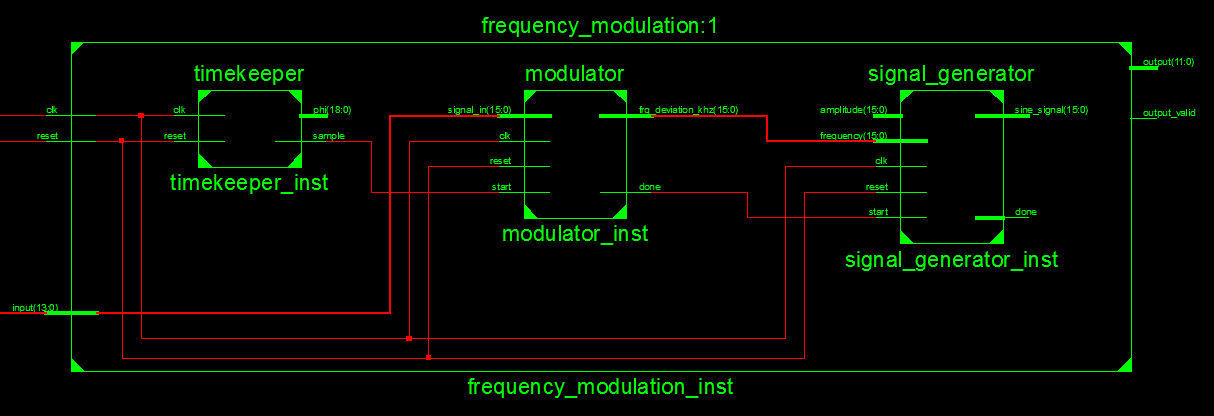
\includegraphics[height=6cm]{images/structure.png}} % importing figure
		\caption{Structural overview of the frequency\_modulation unit} 
		\label{fig:lorem} % labeling to refer it inside the text
	\end{figure} 
\end{landscape}

\subsection{timekeeper}

\begin{adjustwidth}{-0.8cm}{}
	\begin{center}
		\begin{tabular}{ | l | c | l | }
			\hline
			\textbf{Generic} & \textbf{Default} & \textbf{Description} \\
			\hline
			DATA\_WIDTH & 8 & Defines the bit width of the signals in this entity \\
			CLK\_FREQ & 50000000 & Informs the component of the clock speed the desing is running on \\
			BAUD\_RATE & 44000 & Determines the frequency of the sample impulses generated \\
			\hline
		\end{tabular} 
	\end{center}
\end{adjustwidth}

\begin{center}
	\begin{tabular}{ | l | c | l | }
		\hline
		\textbf{Portname} & \textbf{Direction} & \textbf{Description} \\
		\hline
		clk & in & Clock signal \\
		reset & in  & Reset signal \\
		sample & out  & Impulse to be used as start flag for other components \\
		phi & out  & Values between $\pi$ and $-\pi$ to be used for testing \\
		\hline
	\end{tabular} 
\end{center}

The timekeeper unit correlates real time and clock time by using counters.

One counter is used to wait $CLK\_FREQ/BAUD\_RATE$ cycles before raising the output $sample$ to high for one cycle. This signal is used as a start flag for the other components and ensures a constant sample frequency of $BAUD\_RATE$ samples per second.

The other counter is used to wait a certain number of clock cycles, determined by ${DATA\_WIDTH}$ and ${CLK\_FREQ}$, before incrementing an internal signal $phi_int$ by $2^{DATA\_WIDTH - 3}$. This signal is incremented until it reaches pi, when it resets to -pi to count anew. This signal represents $(time \% 2*\pi) - \pi$ and can be used for generating signals with constant frequency during testing.

\subsection{modulator}

\begin{adjustwidth}{-2.7cm}{}
	\begin{center}
		\begin{tabular}{ | l | c | l | }
			\hline
			\textbf{Generic} & \textbf{Default} & \textbf{Description} \\ \hline
			DATA\_WIDTH & 8 & Defines the bit width of the signals in this entity \\
			MAX\_AMPLITUDE & 1.0 & Maximum expected amplitude of the input signal \\
			MIN\_AMPLITUDE & -1.0 & Minimum expected amplitude of the input signal \\
			FREQUENCY\_DEV\_KHZ & 0.5 & Maximum frequency deviation of the carrier rest frequency in kHz \\
			CARRIER\_FREQUENCY\_KHZ & 1.0 & Carrier rest frequency in kHz \\
			\hline
		\end{tabular} 
	\end{center}
\end{adjustwidth}

\vspace{5mm}

\begin{adjustwidth}{-3.7cm}{}
	\begin{center}
		\begin{tabular}{ | l | c | l | }
			\hline
			\textbf{Portname} & \textbf{Direction} & \textbf{Description} \\
			\hline
			clk & in & Clock signal \\
			reset & in  & Reset signal \\
			start & in  & Start flag signals the component that it should start calculations \\
			done & out  & Done bit signals that calculations have been completed and the output is holding valid data \\
			signal\_in & in  & Sample value of the modulation signal \\
			frq\_deviation\_khz & out  & Calculated frequency to be used as input for the signal generator \\
			\hline
		\end{tabular} 
	\end{center}
\end{adjustwidth}

\vspace{4mm}

The modulator takes sample values of the modulation signal and translates them into a frequency. According to \textit{MIN\_AMPLITUDE} and \textit{MAX\_AMPLITUDE} it calculates a mean voltage level. A deviation from this voltage level translates to an increase or decrease of \textit{frq\_deviation\_khz}. Negative deviation of the mean amplitude correlates to a decrease of \textit{frq\_deviation\_khz} and positive deviation results in an increase. If there is no deviation at all the output shows the rest frequency of the carrier provided by the generic \textit{CARRIER\_FREQUENCY\_KHZ}.

\subsection{signal generator}

\begin{center}
	\begin{tabular}{ | l | c | l | }
		\hline
		\textbf{Generic} & \textbf{Default} & \textbf{Description} \\ \hline
		DATA\_WIDTH & 8 & Defines the bit width of the signals in this entity \\
		BAUD\_RATE & 44000.0 & The baudrate of the signal generator \\
		\hline
	\end{tabular} 
\end{center}


\begin{adjustwidth}{-3.3cm}{}
	\begin{center}
		\begin{tabular}{ | l | c | l | }
			\hline
			\textbf{Portname} & \textbf{Direction} & \textbf{Description} \\
			\hline
			clk & in & Clock signal \\
			reset & in  & Reset signal \\
			start & in  & Start flag signals the component that it should start calculations \\
			done & out  & Done bit signals that calculations have been completed and the output is holding valid data \\
			frequency & in  & The frequency of the generated sign signal \\
			amplitude & in  & The amplitde of the generated sign signal \\
			sine\_signal & out  & The current sample of the generated sign signal \\
			\hline
		\end{tabular} 
	\end{center}
\end{adjustwidth}

\vspace{4mm}

The \textit{signal\_generator} is the core component of the design. The component instantiates the \textit{sine\_cordic} component we developed for the first task to generate a continuous set of sine wave samples with frequency and amplitude according to its inputs. These inputs are variable and the frequency of the output signal is determined by the \textit{modulator}.


\subsection{frequency modulation}


\begin{adjustwidth}{-2.6cm}{}
	\begin{center}
		\begin{tabular}{ | l | c | l | }
			\hline
			\textbf{Generic} & \textbf{Default} & \textbf{Description} \\ \hline
			INTERNAL\_DATA\_WIDTH & 16 & Defines the bit width of the signals in this entity \\
			INPUT\_DATA\_WIDTH & 14 & Data width of the ADC register \\
			TIME\_PRECISION & 19 & Time precision data width to be used in the \textit{timekeeper} \\
			OUTPUT\_DATA\_WIDTH & 12 & Data width of the DAC register \\
			CLK\_FREQ & 50000000 & The clock frequency of the design \\
			BAUD\_RATE & 44000.0 & The baudrate of the signal generator \\
			CARRIER\_FREQ & 1.0 & The rest frequency of the carrier signal \\
			FREQUENCY\_DEV\_KHZ & 0.5 & Maximum frequency deviation of the carrier rest frequency in kHz \\
			\hline
		\end{tabular} 
	\end{center}
\end{adjustwidth}

\begin{center}
	\begin{tabular}{ | l | c | l | }
		\hline
		\textbf{Portname} & \textbf{Direction} & \textbf{Description} \\
		\hline
		clk & in & Clock signal \\
		reset & in  & Reset signal \\
		input & in  & Sample of the ADC \\
		output\_valid & out  & Valid data flag to be written to the DAC \\
		output & out  & Output value to be written in the DAC register \\
		\hline
	\end{tabular} 
\end{center}

The frequency modulation component wires all the components together. It connects the sample impulse signals of the \textit{timekeeper} to the input \textit{start} ports of the \textit{modulator}, which in turn starts the \textit{signal\_generator}. It wires the \textit{input} port to the \textit{signal\_in} port of the modulator, the \textit{frq\_deviation\_khz} output port of the \textit{modulator} to the \textit{frequency} input port of the \textit{signal\_generator} and the \textit{sine\_signal} output port of the \textit{signal\_generator} to the \textit{output} port of the \textit{frequency\_modulator}. The \textit{done} output port of the \textit{signal\_generator} is connected to the \textit{output\_valid} output of the \textit{frequency\_modulator}.




